\chapter*{Sobre o Autor}
\addcontentsline{toc}{chapter}{Sobre o Autor}

\begin{minipage}{0.72\textwidth}
Sou o \textbf{Andrey Alencar Quadros}, professor EBTT no Instituto Federal de Rond{\^o}nia, desenvolvedor e pesquisador. Coordeno o \emph{Projeto Cidades Inteligentes Ariquemes — Eixo Sa{\'u}de}. 
Formei-me em \textbf{Ci{\^e}ncia da Computa{\c c}{\~a}o} (UFMT), tenho \textbf{Bacharelado em Teologia} (CESM) e \textbf{Licenciatura em Computa{\c c}{\~a}o} (IFRO). Sou p{\'o}s-graduado (MBA) em \textbf{Governan{\c c}a de TI} (UPF) e \textbf{Marketing Digital} (UniBF), e mestre pelo \textbf{PROFNIT}. 
Escrevo e publico nas interfaces entre f{\'e}, tecnologia e educa{\c c}{\~a}o.
\medskip

Assino livros e artigos como: \emph{Caminhando com Deus na Era da Modernidade L{\'\i}quida} (Clube de Autores, 2023), \emph{O C{\'o}digo do Aprendizado} (2024/25) e estudos em educa{\c c}{\~a}o e tecnologia.
\medskip

\textbf{Contatos e redes}: \url{https://andreyquadros.com.br} \quad Instagram: \texttt{@andreyalencarquadros}
\end{minipage}\hfill
\begin{minipage}{0.24\textwidth}
\centering
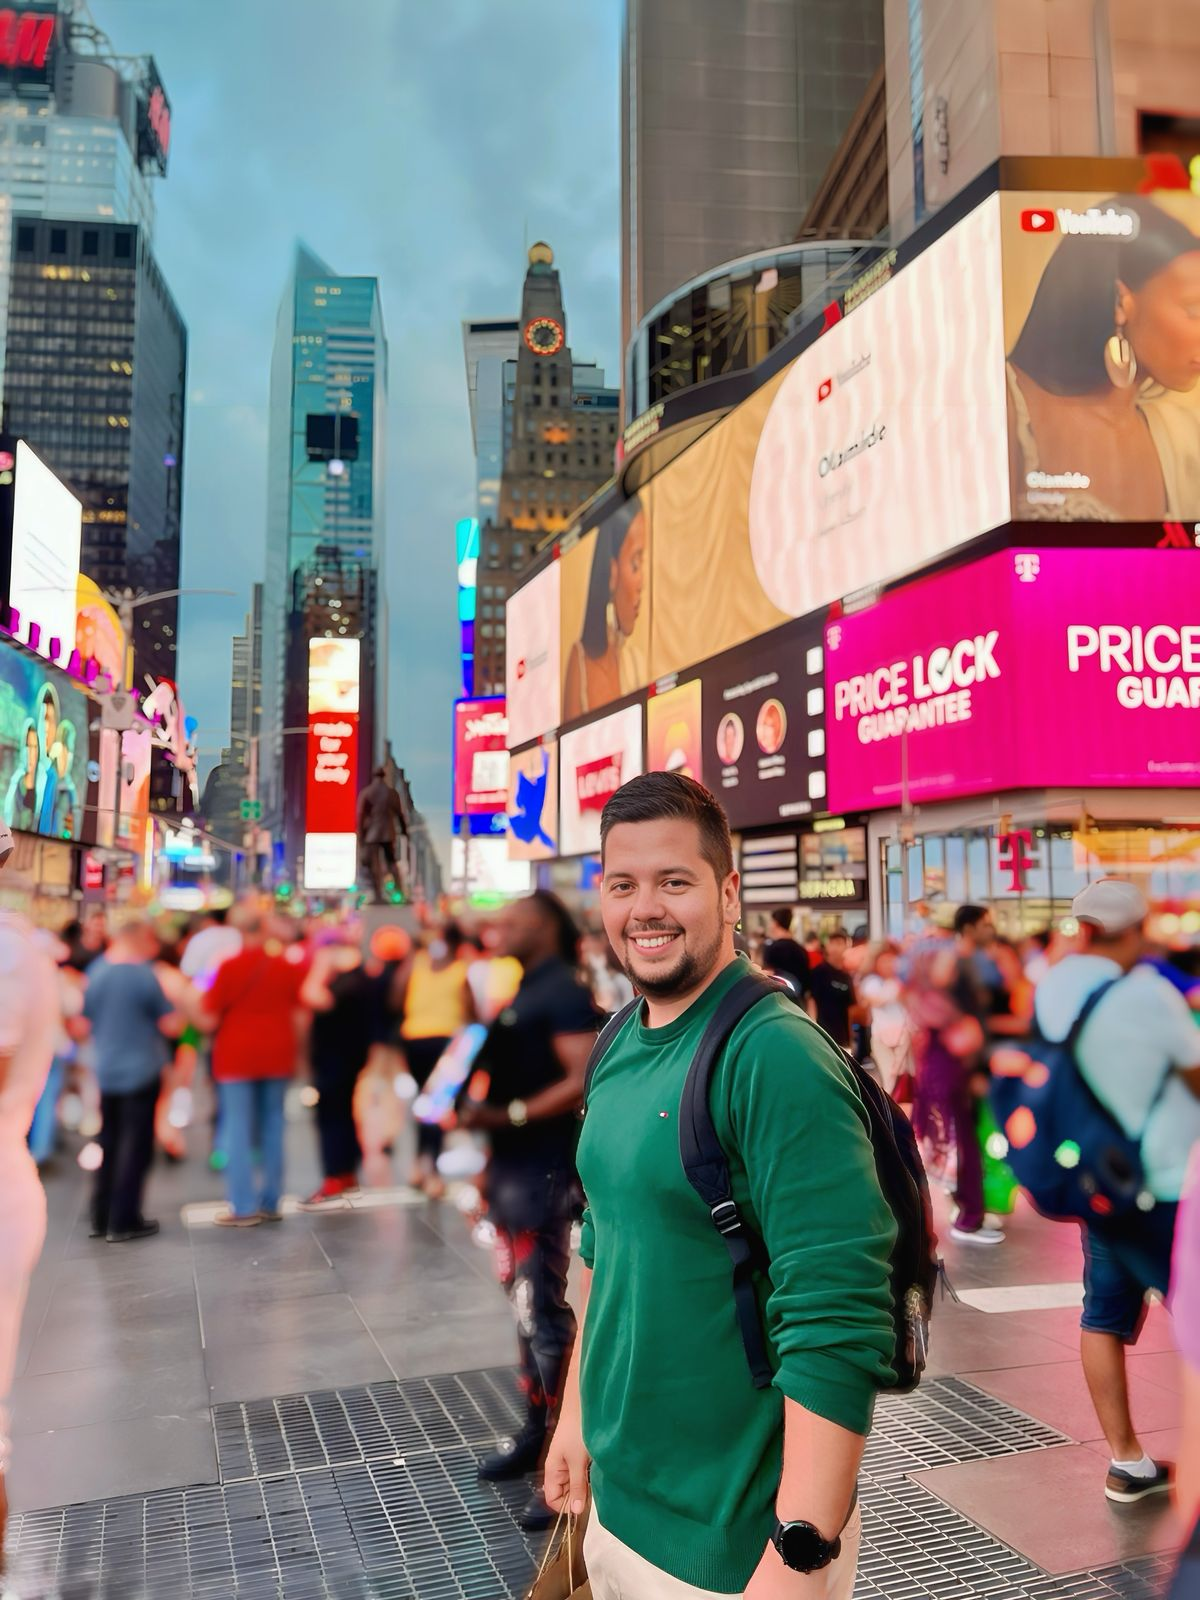
\includegraphics[width=\linewidth]{img/autor.jpg}\\[0.5em]
{\small \textit{(insira sua foto em \texttt{img/autor.jpg})}}\\[1em]

\includegraphics[width=\linewidth]{img/qr_site_placeholder.png}\\[-0.2em]
{\small \textit{QR para o site}}\\
\end{minipage}

% Dica: Se preferir gerar o QR diretamente no \LaTeX, inclua no preambulo:
% \usepackage{qrcode}
% e, aqui, substitua a imagem acima por: \qrcode[height=2.8cm]{https://andreyquadros.com.br}
